\documentclass{article}

\usepackage[italian]{babel}
\usepackage[utf8]{inputenc}


\usepackage{listings} % for coding like part

\usepackage{graphicx}
\graphicspath{ {./images/} }

\usepackage{float} %#$@&*!

\usepackage{hyperref} % lasciare per ultimo
 
% huge indentation of paragraph only for demonstration purposes. 
%\setlength{\parindent}{5em} 
% some paragraph skip to better distinguish  lines of different paragraphs  
\setlength{\parskip}{.8em} 

\begin{document}
\begin{titlepage}
	\begin{center}
		\Huge{Progetto Basi di Dati}\\
		[20mm]
		\Large{Paolo Addis}\\
		\Large{Samuele Poz}\\
		\Large{Tristano Munini}\\
		[20mm]
		\Large{RENDERE CARINO}
	\end{center}
\end{titlepage}

\tableofcontents
\thispagestyle{empty} 
\cleardoublepage
\setcounter{page}{1}

% REGOLE DI STILE
% - scrivere in modo impersonale no "abbiamo deciso di"
% - 


% TODO
% - abbellire hyperlinks
% - modifiche su full_er_model_02
% - rimuovere CARTELLA-CLINICA dallo schema ER della Progettazione ER
% - CARTELLA-CLINICA in DIAGNOSI-EFFETTUATA o altro


% TODO -- SCHEMI 
% - primo schema: pazinete fuori regione, attributi composti multivalore, no cartella clinica 
% - secondo schema: togli ternaria, toglie specializzazione, togli attributi composti, multivalore 
% - terzo schema: per prestazioni aggiungiamo EFFETTUATA A 

% COSE DA RICORDARE
% NEI REQUISITI
% - aggiungere numero di accessi effettuati e numero di Pazienti, Ricovero, ecc
% - Evidenziare la necessità dell'ospedale di accedere spesso alle diagnosi di un dato paziente


\section{Progettazione Concettuale}\label{sec:prog_conc}

\subsection{Raccolta ed Analisi dei Requisiti}

Si vuole modellare il seguente insieme di informazioni riguardanti un sistema
per la gestione delle diagnosi e delle terapie dei pazienti ricoverati in un
dato ospedale.
\begin{itemize}
  \item Di ogni ricovero, il sistema deve memorizzare il codice univoco, il 
        nome della divisione ospedaliera (Cardiologia, Reumatologia, Ortopedia,
        \dots ), il paziente ricoverato, le date di inizio e fine del ricovero 
        e il motivo principale del ricovero.

  \item Di ogni paziente, il sistema deve memorizzare il codice sanitario 
        (univoco), il cognome, il nome, la data di nascita, il luogo di nascita 
        e la provincia di residenza. Per i pazienti residenti fuori regione, 
        vengono memorizzati anche il nome della ULSS e la regione di appartenenza.
        Inoltre, per ogni paziente, è necessario memorizzare il totale delle
        durate dei ricoveri.

  \item Di ogni diagnosi effettuata durante il ricovero del paziente, sono 
        memorizzati la patologia diagnosticata, col suo codice ICD10 
        (classificazione internazionale delle patologie) e l’indicazione della
        sua gravità (grave: si/no), la data e il nome e cognome del medico che 
        ha effettuato la diagnosi.

  \item Nella base di dati si tiene traccia delle terapie prescritte ai pazienti
        durante il ricovero. Di ogni terapia, si memorizzano il farmaco prescritto,
        la dose giornaliera, le date di inizio e di fine della prescrizione, la 
        modalità di somministrazione ed il medico che ha prescritto la terapia.

  \item Di ogni farmaco sono memorizzati il nome commerciale (univoco), l’azienda
        produttrice, il nome e la quantità dei principi attivi contenuti e la 
        dose giornaliera raccomandata.

  \item Si tiene, infine, traccia delle diagnosi che hanno motivato le terapie.
        In particolare, ogni terapia è prescritta al fine di curare una o più 
        patologie diagnosticate. Può capitare anche che una nuova patologia 
        (registrata come nuova diagnosi) sia causata, come effetto collaterale, 
        da una terapia precedentemente prescritta. Tale legame causa-effetto va
        registrato nella base di dati.
\end{itemize}
Tramite un portale web dovrà essere possibile accedere a tale base di dati ed
aggiungere o rimuovere pazienti, ricoveri, diagnosi con relative terapie e farmaci.
% TODO aggiungere numeri/necessità dell'ospedale 


\clearpage
\subsection{Progettazione del Modello E-R}
%TODO
% - A relazione conclusa decidere se aggiungere schemi parziali
% - Descrizione procedimento Inside-Out 
% . Descrizione testuale delle relazioni e entità
Inizialmente l'attenzione è stata concentrata sulle entità PAZIENTE e RICOVERO
in quanto ritenute fondamentali: si può dire che in assenza di un'entità che
rappresenti i pazienti, l'intera base di dati perderebbe significato.  Infatti
per ogni ricovero o diagnosi deve essere possibile risalire al soggetto che è
stato ricoverato o a cui è stata effettuata una diagnosi, altrimenti non si
potrebbero utilizzare correttamente le informazioni raccolte in passato.
RICOVERO, invece, segna i momenti in cui il paziente raggiunge e lascia la
struttura ospedaliera, inoltre permette di indicare in modo univoco le visite e
le cure alle quali è stato sottoposto durante questo periodo.  Le due entità
sono in relazione tra di loro attraverso una VIENE-RICOVERATO che intuitivamente
collega una entità PAZIENTE a molte entità RICOVERO.  È stata poi costruita la
tripletta FARMACO, SOMMINISTRATO-DURANTE e TERAPIA composta rispettivamente da:
un'entità che rappresenta il farmaco con i relativi attributi; una relazione che
permette di indicare che farmaco viene usato durante una terapia; infine
un'entità che raccoglie i dettagli della terapia, ad esempio la dose giornaliera
di farmaco da assumere.  L'entità DIAGNOSI e le rimanenti relazioni, in
particolare CAUSA-EFFETTO, verranno analizzate successivamente.










Progettazione:

Il primo passo della costruzione dello schema E-R è stato l'individuazione
delle entità. Seguendo l'analisi dei requisiti, la prima entità modellata è 
stata RICOVERO che memorizza tutte le informazioni relative a un ricovero e
possiede come attributi: \textit{Codice Ricovero}, \textit{Divisione 
Ospedaliera}, \textit{Paziente Ricoverato}, \textit{Data Inizio}, \textit{Data
Fine}, \textit{motivo}. In particolare, l'attributo \textit{Codice Ricovero} 
è stato scelto come chiave primaria a causa della sua proprietà di unicità. 
Successivamente è stata modellata l'entità PAZIENTE che è ritenuta fondamentale 
in quanto senza di essa la base di dati perderebbe di significato. Per questa 
entità sono stati creati i seguenti attributi: \textit{Codice Sanitario}, 
\textit{Cognome}, \textit{Nome}, \textit{Data di Nascita}, \textit{Luogo di 
Nascita} e \textit{Provincia di residenza} del paziente. E' richiesto inoltre 
di memorizzare informazioni aggiuntive per i pazienti fuori regione. Per far 
ciò è stata creata una specializzazione PAZIENTE-FUORI-REGIONE di PAZIENTE 
i cui attributi sono: \textit{Regione di Appartenenza} e \textit{ULSS}.

1) Paziente
2) Ricovero
3) Viene ricoverato
4) Diagnosi
5) Effettuata durante 
6) Terapia 
6.1) Medico
7) Farmaco 
8) Somministra 
9) Motiva Terapia 











































\subsubsection{Le Entità} % TODO sarebbe meglio creare subsubsubsection o paragrafi per ogni entità?
\begin{itemize}
    \item PAZIENTE: dai requisiti è possibile individuare le seguenti voci
          significative: \textit{codice sanitario}, \textit{cognome},
          \textit{nome}, \textit{data di nascita}, \textit{luogo di nascita} e
          \textit{provincia di residenza} del paziente.
          Per ognuna di esse è stato creato un attibuto. Il codice fiscale
          (d'ora in poi detto anche CF) è stato selezionato come chiave
          primaria in quanto,
          come definito nei requisiti, univoco\footnote{Proprietà fondamentale
          di un attributo per la definizione di esso come chiave primaria.}.
          %Ricordiamo la definizione di chiave primaria univoca e sottoinsieme minimo TODO
          Per salvare gli attributi esclusivi per i pazienti fuori regione
          riguardanti il nome della ULSS e la regione di appartenenza, è stata
          creata l'entità PAZIENTE-FUORI-REGIONE, specializzazione dell'entità
          precedente.  Poiché solo una frazione dell'insieme dei pazienti sarà
          di questo tipo la specializzazione è parziale.
          % TODO aggiungere attributo derivato

    \item RICOVERO: dai requisiti è possibile individuare le seguenti voci 
          significative: \textit{codice ricovero, divisione ospedaliera, 
          paziente ricoverato, data inizio, data fine, motivo} del ricovero. 
          Per ognuna di esse è stato creato un attributo, fatta eccezione per 
          \textit{paziente ricoverato}. Quest'ultima informazione verrà
          memorizzata attraverso la relazione VIENE-RICOVERATO, descritta 
          in seguito. Il \textit{codice ricovero} è stato selezionato come
          chiave primaria dell'entità in quanto univoco.
          
    \item DIAGNOSI: dai requisiti è possibile individuare le seguenti voci 
          significative: \textit{patologia diagnosticata, codice patologia,
          gravità patologia, data, medico}. Per ognuna di esse è stato 
          creato un attributo. In particolare \textit{patologia} è un 
          attributo composto che si suddivide in \textit{codice} e 
          \textit{gravità}. Si assume che la data comprenda anche l'ora in 
          cui è stata effettuata la diagnosi. DIAGNOSI è un'entità debole 
          in quanto la chiave primaria è definita attraverso l'attributo
          \textit{data} e la relazione EFFETTUATA-DURANTE. La chiave è
          stata stabilita sfruttando l'assunzione precedente rigurado la 
          data in modo tale che per ogni ricovero non sia possibile 
          associare più diagnosi effettuate nello stesso istante.

    \item FARMACO: dai requisiti è possibile individuare le seguenti voci
          significative: \textit{nome commerciale, azienda produttrice, 
          nome principi attivi, quantità principi attivi, dose giornaliera
          raccomandata}. Per ognuna di esse è stato creato un attributo. In
          particolare \textit{nome principi attivi e quantità principi 
          attivi} sono attributi multivalore e la chiave primaria è 
          rappresentata da \textit{nome commerciale} in quanto univoco.
          
    \item TERAPIA: dai requisiti è possibile individuare le seguenti voci
          significative: \textit{farmaco prescritto, dose giornaliera, 
          modalità di somministrazione, medico prescrivente}. 
          Sono stati definiti gli attributi \textit{dose giornaliera} e 
          \textit{modalità somministrazione} mentre l'informazione relativa
          alle altre voci verrà considerata in altre entità e relazioni.
          In particolare il medico prescrivente, le date di inzio e fine 
          della terapia verranno gestite nella relazione MOTIVA-TERAPIA,
          in quanto la terapia è intesa come metodo per la sommistristrazione 
          di un farmaco al fine di curare una patologia. La 
          chiave primaria è composta dagli attributi di terapia e dalla
          relazione SOMMINISTRA che rende l'entità un'entità debole e consente 
          di mantenere i dati relativi al farmaco prescritto.



\end{itemize}

\subsubsection{Le Relazioni}
\begin{itemize}
    \item VIENE-RICOVERATO: un tipo di relazione Uno-A-Molti tra PAZIENTE e
          RICOVERO. Entrambe le partecipazioni sono totali.
    
    \item EFFETTUATA-DURANTE: un tipo di relazione Uno-A-Molti tra DIAGNOSI 
          e RICOVERO. La partecipazione di RICOVERO è parziale mentre quella
          di DIAGNOSI è totale.

    \item SOMMINISTRA: un tipo di relazione Uno-A-Molti tra FARMACO e TERAPIA.
          La partecipazione di FARMACO è parziale mentre quella di
          TERAPIA è totale.
    
    \item MOTIVA-TERAPIA: una relazione ternaria in cui partecipano le entità
          TERAPIA e DIAGNOSI in una meccanica di causa-effetto. Possiede i
          seguenti attributi \textit{medico prescrivente, data inizio, data  fine}. 
          L'entità DIAGNOSI partecipa con cardinalità (0,1) mentre TERAPIA 
          partecipa con cardinalità (1,N).
\end{itemize}      
            
                 

% TODO Immagine diagnosi, terapia SENZA attributi e motiva terapia con attributi 
% Senza ricorsione e con ricorsione
Nella costruzione della relazione MOTIVA-TERAPIA si è fatta particolare
attenzione all'ultimo punto dell'analisi dei requisiti in cui si specifica che
una terapia può essere associata ad una diagnosi in due modi differenti: quello
che la definisce come cura per una patologia e quello che la definisce come
causa di una nuova patologia.  Va sottolineato che in entrambi i casi, nella
base di dati, la patologia è salvata attraverso DIAGNOSI.

In un primo momento è stato modellato il sottoschema illustrato in Figura
\ref{schema_piccolo1}.  Il modo in cui è stata definita l'entità TERAPIA
permetterà di modellare il requisito \textit{ogni terapia può curare più
patologie}.  Un'informazione come data di inizio, o data di fine, o medico
prescrivente, non può essere memorizzata in TERAPIA perché, altrimenti, non
sarebbe possibile applicare questa stessa terapia in uno spazio temporale
differente, pena la perdita delle informazioni precedenti. D'altra parte non è
nemmeno accettabile includere nella chiave primaria le informazioni relative
alle date ed al medico, perché così facendo si differenzierebbero le entità,
andando contro il requisito che si vole modellare.  Da qui la necessità di
omettere attributi data inizio, data fine e medico prescrivente in TERAPIA,
assegnandoli alla relazione MOTIVA-TERAPIA.  Intuitivamente questi attributi
riguardano contemporaneamente la DIAGNOSI, quindi la patologia che si vuole
curare, e la TERAPIA applicata, quindi il modo in cui si vuole affrontare la
patologia, definendone il periodo in cui la terapia viene applicata e chi ha
definito questo periodo.  Nei requisiti è specificato che per alcune patologie
manchino le cure, per questo motivo la partecipazione a MOTIVA-TERAPIA di
DIAGNOSI è parziale.  Invece è sensato pensare che se una terapia esiste possa
curare almeno una patologia, la partecipazione di TERAPIA quindi è totale.  Nel
complesso MOTIVA-TERAPIA, per ora, risulta essere una relazione Uno-A-Molti:
nel testo è specificato che ad ogni diagnosi possa essere associata al più una
terapia; mentre TERAPIA è stata definita appositamente per poter esser
associata a più DIAGNOSI.

\begin{figure}[!ht] % TODO abbellire 
      \centering 
      \begin{minipage}{.5\textwidth}

\centering 
            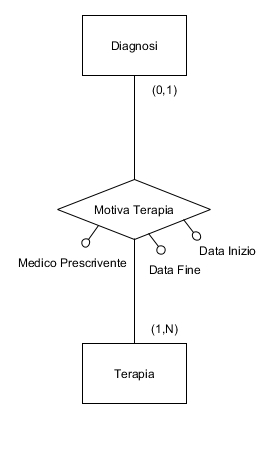
\includegraphics[width=\linewidth]{piccolo1} \caption{Prima
modellazione} \label{schema_piccolo1} \end{minipage}%
\begin{minipage}{.5\textwidth} \centering
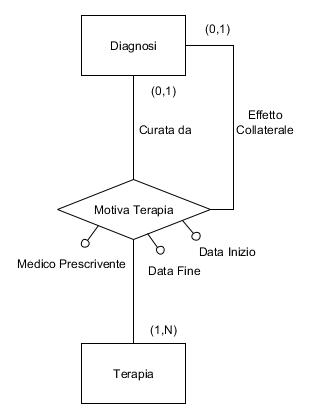
\includegraphics[width=\linewidth]{piccolo2} \caption{Relazione completa}
\label{schema_piccolo2} \end{minipage} \end{figure}

Ora è necessario modellare la situazione in cui una terapia prescritta è causa
di una nuova patologia.  L'informazione che si vuole mantenere non dipende
esclusivamente dall'entità TERAPIA, dipende anche dal periodo di applicazione,
quindi non è sufficiente creare una nuova relazione tra TERAPIA e DIAGNOSI.  La
soluzione migliore è quella di trasformare MOTIVA-TERAPIA in una relazione
ternaria: con DIAGNOSI che partecipa da una parte come patologia in cura e
dall'altra come rilevazione di una nuova patologia.  Per comodità, il risultato
di tale trasformazione è riportato in Figura \ref{schema_piccolo2}.  Ricordando
che non tutte le applicazioni di una terapia causano un effetto collaterale e
che ne possono causare al massimo uno, la partecipazione di DIAGNOSI come
effetto collaterale è parziale con cardinalità 1.

A questo punto è necessario introdurre dei vincoli d'integrità:
\begin{itemize}
  \item in ogni tripletta di MOTIVA-TERAPIA non può comparire due volte la
    stessa DIAGNOSI;
  \item la DIAGNOSI che partecipa come effetto collaterale deve avere una data
    successiva alla data della prima diagnosi.
\end{itemize}
%TODO ho dimenticato qualcosa??
Nella fase logica verrà mostrato che questa relazione può essere trasformata,
senza perdita d'informazione, e con l'aggiunta di una nuova entità, in
relazioni binarie.


\begin{figure}[H] % TODO abbellire
    \centering
    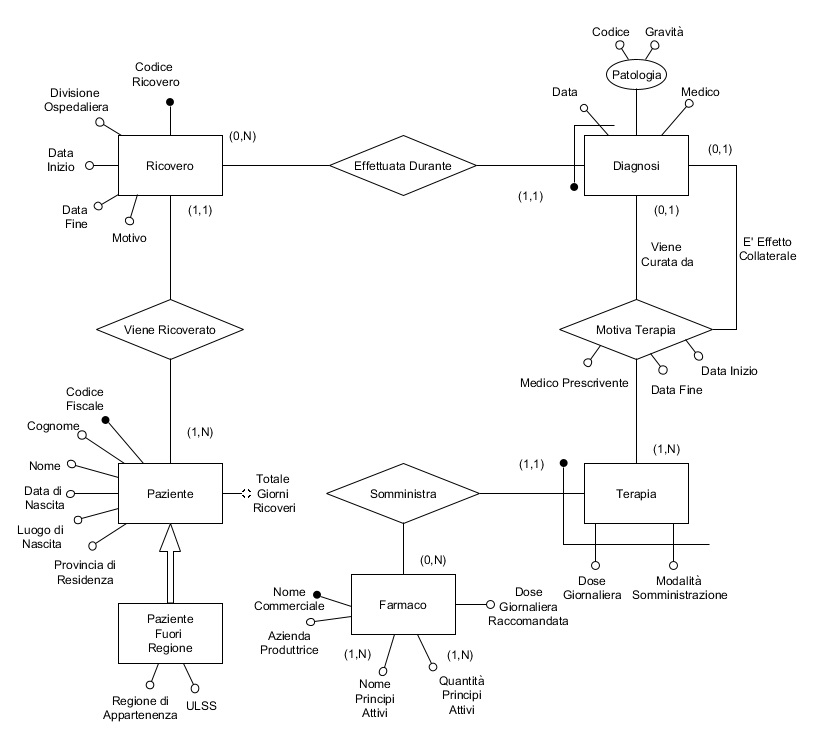
\includegraphics[width=\linewidth]{schema1}
    \caption{Lo schema Entità-Relazioni completo}
    \label{schema_ER_progettazione_modello}
\end{figure}


%\begin{figure}[h] % TODO abbellire
%\caption{Entità PAZIENTE con specializzazione e, a destra, RICOVERO}
%
\includegraphics[width=0.4\textwidth]{galaxy}
%
\includegraphics[width=0.4\textwidth]{galaxy}
%\end{figure}




\clearpage
\section{Progettazione Logica}

%TODO
%Cose che si potrebbero aggiungere:
% - Partizionamento di una relazione (si può fare con MEDICO collegato a PAZIENTE e DIAGNOSI)
%   (secondo Tri 'fare solo se non abbiamo abbastanza materiale')

\subsection{Ristrutturazione del Modello E-R}
\subsubsection{Semplificazione dei Concetti}
%% logical design steps
% ristrutturazione semplificare ER
% schema ristrutturato
% ottimizzazione analisi ridondanze
% schema con ridondanza
% elenco tabelle
% vincoli d'integrità

È utile semplificare strutture come specializzazioni, attributi composti e
attributi multivalore perché renderà più facile la traduzione del modello
Entità-Relazioni in quello Relazionale.

Ricordando che quest'ultimo non permette di rappresentare generalizzazioni sarà
necessario rimuovere tutte le specializzazioni dal nostro schema E-R.  Si può
notare che la specializzazione PAZIENTE-FUORI-REGIONE può essere facilmente
rappresentata aggiungendo due attributi all'entità PAZIENTE.  I nuovi
attributi, \textit{ULSS} e \textit{Regione di Appartenenza}, in PAZIENTE
saranno facoltativi poiché la specializzazione è parziale.  La rimozione delle
generalizzazioni non è sempre così immediata: se PAZIENTE-FUORI-REGIONE avesse
avuto una relazione in più rispetto al genitore si sarebbero dovute valutare
varie opzioni.  Per esempio la creazione di una nuova relazione per
simboleggiare il legame tra genitore e figlio, lasciando invariati gli
attributi.  Oppure la duplicazione nel figlio di tutti gli attributi e di tutte
le relazioni del genitore.  

Anche nel caso degli attributi composti la semplificazione è immediata, infatti
nello schema l'unico attributo composto è \textit{Patologia} in DIAGNOSI.  Può
essere trasformato in due nuovi attributi \textit{Codice Patologia} e
\textit{Gravità Patologia} che contengono esattamente la stessa informazione.

Bisogna prestare più attenzione agli attributi multivalore: in FARMACO sono
presenti \textit{Nome Principi Attivi} e \textit{Quantità Principi Attivi}
entrambi obbligatori e multivalore.  L'unica semplificazione attuabile è creare
una nuova entità chiamata PRINCIPIO-ATTIVO è metterla in relazione
Molti-A-Molti con FARMACO attraverso la nuova relazione CONTIENE.
PRINCIPIO-ATTIVO avrà un solo attributo, scelto anche come chiave primaria,
chiamato \textit{Nome}, mentre alla relazione CONTIENE verrà aggiunto
l'attributo \textit{Quantità}.  In questo modo saranno modellate esattamente le
stesse informazioni precedentemente modellate dagli attributi multivalore.
Rimozione t Scelta della chiavi primarie








\begin{figure}[H] % TODO abbellire
  \centering
  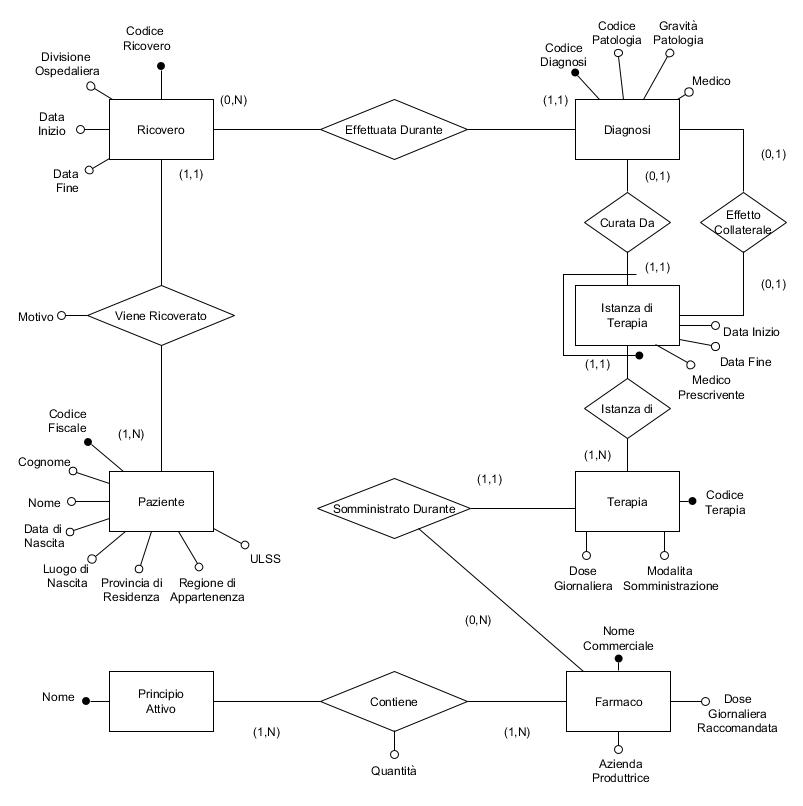
\includegraphics[width=\linewidth]{schema2.jpg}
  \caption{Lo schema Entità-Relazioni completo}
  \label{schema_ER_ristrutturato}
\end{figure}

% TODO NELLA FASE LOGICA
% - verrà aggiunta relazione tra PAZIENTE DIAGNOSI (es EFFETTUATA A) per verificare la differenza di prestazioni
% - l'unica ridondanza è data da EFFETTUATA A, la ricorsione DIAGNOSI->DIAGNOSI (o ISTANZA DI TERAPIA -> DIAGNOSI) NON è ridondanza (esprime informazioni differenti)


\clearpage
\subsubsection{Analisi delle Ridondanze}

Lo schema Entità-Relazioni  \autoref{schema_ER_ristrutturato} % TODO quanità di giorni che ricoverato


Visto il requisito di stampa delle diagnosi effettuate da un singolo paziente, ai fini di ottimizzazione consideriamo l'inserimento della relazione:
\begin{itemize}
\item EFFETTUATA A: una relazione Uno-A-Molti tra PAZIENTE 
          e DIAGNOSI. La partecipazione di PAZIENTE è parziale mentre quella
          di DIAGNOSI è totale. 
\end{itemize}

Viene creato quindi il ciclo in \autoref{fig:ciclo-ridondanza} PAZIENTE, RICOVERO, DIAGNOSI dato dalle relazioni VIENE RICOVERATO, EFFETTUATA DURANTE, EFFETTUATA A.

\begin{figure}[H] % TODO abbellire
      \centering
      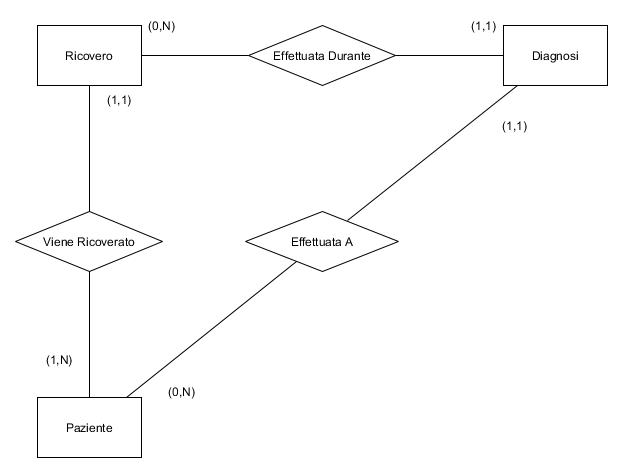
\includegraphics[width=\linewidth]{schema3.jpg}
      \caption{Ciclo con ridondanza}
      \label{fig:ciclo-ridondanza}
    \end{figure}
Procediamo a valutare se è conveniente mantenere la relazione EFFETTUATA A tra PAZIENTE e DIAGNOSI in funzione della frequenza delle operazioni di inserimento nuove diagnosi e stampa dello storico diagnosi di un paziente.

% TODO REQUISITO specificare nei requisiti le operazioni richieste e i volumi

Riportiamo i volumi stimati durante la fase dei requisiti in \autoref{tab:volumi-ciclo} e la frequenza delle operazioni interessate in \autoref{tab:operazioni-ciclo}.

% TODO REQUISITO spostare table:volumi nei requisiti
\begin{table}[H]
	\label{tab:volumi}
	\centering
	\begin{tabular}{|l|c|r|}
		\hline
		\textbf{Concept}      & \textbf{Type} & \textbf{Volume} \\ \hline
		Paziente              & E             & 100000          \\ \hline
		Ricovero              & E             & 300000          \\ \hline
		Diagnosi              & E             & 1200000         \\ \hline
		Terapia               & E             & 30000           \\ \hline
		Istanza di Terapia    & E             & 1200000         \\ \hline
		Farmaco               & E             & 10000           \\ \hline
		Viene Ricoverato      & R             & 300000          \\ \hline
		Effettuata Durante    & R             & 1200000         \\ \hline
		Effettuta A           & R             & 1200000         \\ \hline
		Curata Da             & R             & 1200000         \\ \hline
		Istanza Di            & R             & 1200000         \\ \hline
            Effetto Collaterale   & R             & 50000           \\ \hline
		Somministrato Durante & R             & 10000           \\ \hline
	\end{tabular}
	\caption{Tabella dei volumi}
\end{table}

\begin{table}[H]
	\label{tab:volumi-ciclo}
	\centering
	\begin{tabular}{|l|c|r|}
		\hline
		\textbf{Concept}   & \textbf{Type} & \textbf{Volume} \\ \hline
		Paziente           & E             & 100000          \\ \hline
		Ricovero           & E             & 300000          \\ \hline
		Diagnosi           & E             & 1200000         \\ \hline
		Viene Ricoverato   & R             & 300000          \\ \hline
		Effettuata Durante & R             & 1200000         \\ \hline
		Effettuata A       & R             & 1200000         \\ \hline
	\end{tabular}
	\caption{Tabella dei volumi ridotta}
\end{table}

\begin{table}[H]
	\label{tab:operazioni-ciclo}
	\centering
	\begin{tabular}{|l|c|r|}
		\hline
		\textbf{Operation}      & \textbf{Type} & \textbf{Frequency} \\ \hline
		Inserimento Diagnosi    & I             & 700/giorno         \\ \hline
		Stampa Storico Diagnosi & I             & 1400/giorno        \\ \hline
	\end{tabular}
	\caption{Tabella delle operazioni ridotta}
\end{table}

Nel caso con ridondanza per l'operazione di inserimento di una nuova diagnosi sono necessari 1 accesso in scrittura per l'entità DIAGNOSI e 1 accesso in scrittura per entrambe le relazioni EFFETTUATA DURANTE e EFFETTUATA A.
Per l'operazione di stampa delle diagnosi di un paziente sono necessari 12 accessi in lettura per la relazione EFFETTUATA A e 12 accessi in lettura per l'entità DIAGNOSI.

Considerando il costo di 1 accesso in scrittura come 2 accessi in lettura, calcoliamo il numero di accessi complessivo giornaliero per le 2 operazioni nel caso con ridondanza:
\begin{equation}
  3W \times 700 + 24R \times 1400 \approx	37800R
\end{equation}

\begin{table}[H]
	\label{table:3}
	\centering
	\begin{tabular}{|l|c|c|c|}
		\hline
		\textbf{Concept}    & \textbf{Type} & \textbf{Access} & \textbf{Type} \\ \hline
		\multicolumn{4}{|c|}{Inserimento Diagnosi}                            \\ \hline
		Diagnosi            & E             & 1               & W             \\ \hline
		Effettutata Durante & R             & 1               & W             \\ \hline
		Effettuata A        & R             & 1               & W             \\ \hline
		\multicolumn{4}{|c|}{Stampa Storico Diagnosi}                         \\ \hline
		Effettuata A        & R             & 12              & R             \\ \hline
		Diagnosi            & E             & 12              & R             \\ \hline
	\end{tabular}
	\caption{Tabella dei costi, caso con ridondanza}
\end{table}

Nel caso senza ridondanza per l'operazione di inserimento di una nuova diagnosi sono necessari 1 accesso in scrittura per l'entità DIAGNOSI e 1 accesso in scrittura per la relazione EFFETTUATA DURANTE.
Per l'operazione di stampa delle diagnosi di un paziente sono necessari 3 accessi in lettura per la relazione VIENE RICOVERATO, 12 accessi in lettura per la relazione EFFETTUATA DURANTE e 12 accessi in lettura per l'entità DIAGNOSI.

Considerando il costo di 1 accesso in scrittura come 2 accessi in lettura, calcoliamo il numero di accessi complessivo giornaliero per le 2 operazioni nel caso senza ridondanza:
\begin{equation}
  2W \times 700 + 27R \times 1400 \approx	40600R
\end{equation}

\begin{table}[H]
	\label{table:4}
	\centering
	\begin{tabular}{|l|c|c|c|}
		\hline
		\textbf{Concept}    & \textbf{Type} & \textbf{Access} & \textbf{Type} \\ \hline
		\multicolumn{4}{|c|}{Inserimento Diagnosi}                            \\ \hline
		Diagnosi            & E             & 1               & W             \\ \hline
		Effettutata Durante & R             & 1               & W             \\ \hline
		\multicolumn{4}{|c|}{Stampa Storico Diagnosi}                         \\ \hline
		Viene Ricoverato    & R             & 3               & R             \\ \hline
		Effettutata Durante & R             & 12              & R             \\ \hline
		Diagnosi            & E             & 12              & R             \\ \hline
  \end{tabular}
  \caption{Tabella dei costi, caso senza ridondanza}
\end{table}

Concludiamo che è conveniente mantenere la ridondanza visto il costo minore delle operazioni giornaliere.

\subsection{Traduzione da ER a Relazionale}



%% sotto un copia-incolla da vecchio file %%

% SCRIVIAMO LA LISTA DELLE TABELLE CON TUTTE LE CHIAVI BELLE DENTRO 
% SOTTO SCRIVIAMO LA LISTA: "LA RELAZIONE X è GARANTITA DA QUESTA COMBO 
%                            DI CHIAVI (Y,Z)..."
% 
% - Traduzione di VIENE-RICOVERATO (da scrivere bene perchè è la prima)
% 
% PAZIENTE (_CF_, NOME,...)
% RICOVERO (_CODICE-RICOVERO_,...,DIVISIONE-OSPEDALIERA, CF, MOTIVO)
%           . CF chiave esterna not null, 
%           . MOTIVO not null
% . Specificare che la traduzione cattura la partecipazione (0,N)(1,1)
%   e non (1,N)(1,1), bisogna introdurre un vincolo esterno per garantire
%   (1,N)
% 
% - Traduzione di EFFETTUATA-DURANTE 
%   . lo creiamo aggiungendo una chiave esterna su DIAGNOSI con not null
% 
% - Traduzione di CARTELLA-CLINICA
%   . lo creiamo aggiungendo una chiave esterna su DIAGNOSI con not null
% 
% - Traduzione di SOMMINISTRATO-DURANTE
%   . lo creiamo aggiungendo una chiave esterna su TERAPIA con not null
% 
% - Traduzione di CURATA-DA e di ISTANZA-DI e EFFETTO-COLLATERALE
%   . ISTANZA-DI-TERAPIA (__DIAGNOSI_,_TERAPIA__,...,DIAGNOSI-EC) 
%   DIAGNOSI e TERAPIA e DIAGNOSI-EC sono chiavi esterne.
%   La coppia DIAGNOSI e TERAPIA è chiave. 
%   Si deve inserire UNIQUE per DIAGNOSI e non per la coppia per 
%   garantire (1,1).      
%   Si deve inserire un vincolo esterno per garantire (1,N) su terapia
%   Si deve inserire UNIQUE su DIAGNOSI-EC per garantire 1 tra DIAG e EC




\clearpage
\section{Progettazione Fisica}
\subsection{Nuovi Indici}
% Indice possibile è provincia 



\clearpage
\section{Definizione della Base di Dati in SQL}
\subsection{Definizione delle Tabelle}
\subsection{Definizione di Query Significative}




\clearpage

\section{Analisi Dati}
\subsection{Popolamento della Base di Dati}
\subsection{Analisi Dati in R}



\clearpage
\section{Portale Web}
\subsection{Interfaccia Grafica}
\subsection{Comunicare con pgAdmin}



\end{document}

\cleardoublepage
% Code example
\begin{lstlisting}[language=bash,title={bash version}]
#!/bin/bash
echo "Hello , world!"
\end{lstlisting}
